\section{eo\-FDCFile\-Snapshot$<$ EOT $>$ Class Template Reference}
\label{classeo_f_d_c_file_snapshot}\index{eoFDCFileSnapshot@{eoFDCFileSnapshot}}
Specific class for FDCStat monitoring: As I failed to have FDC stat as an {\bf eo\-Stat}{\rm (p.\,\pageref{classeo_stat})}, this is the trick to put the 2 {\bf eo\-Param}{\rm (p.\,\pageref{classeo_param})}$<$std::vector$<$double$>$ $>$ into a monitor This class does nothing else.  


{\tt \#include $<$eo\-FDCStat.h$>$}

Inheritance diagram for eo\-FDCFile\-Snapshot$<$ EOT $>$::\begin{figure}[H]
\begin{center}
\leavevmode
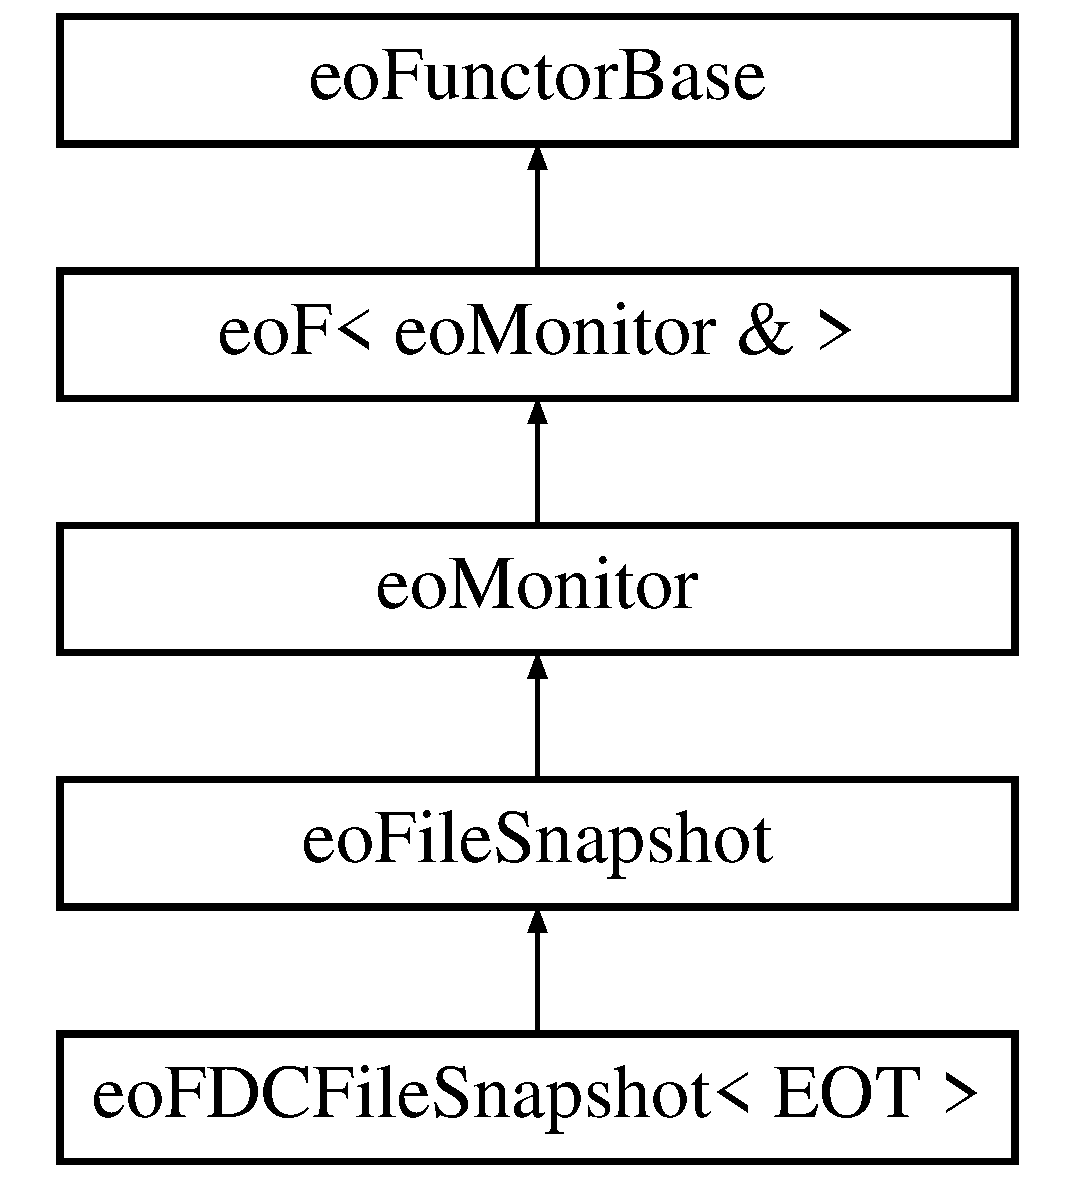
\includegraphics[height=5cm]{classeo_f_d_c_file_snapshot}
\end{center}
\end{figure}
\subsection*{Public Member Functions}
\begin{CompactItemize}
\item 
{\bf eo\-FDCFile\-Snapshot} ({\bf eo\-FDCStat}$<$ {\bf EOT} $>$ \&\_\-FDCstat, std::string \_\-dirname=\char`\"{}tmp\-FDC\char`\"{}, unsigned \_\-frequency=1, std::string \_\-filename=\char`\"{}FDC\char`\"{}, std::string \_\-delim=\char`\"{} \char`\"{})
\begin{CompactList}\small\item\em Ctor: in addition to the parameters of the ctor of an {\bf eo\-File\-Snapshot}{\rm (p.\,\pageref{classeo_file_snapshot})} we need here an {\bf eo\-FDCStat}{\rm (p.\,\pageref{classeo_f_d_c_stat})}. \item\end{CompactList}\item 
virtual void {\bf add} (const {\bf eo\-Param} \&\_\-param)\label{classeo_f_d_c_file_snapshot_a1}

\begin{CompactList}\small\item\em just to be sure the add method is not called further \item\end{CompactList}\end{CompactItemize}
\subsection*{Private Attributes}
\begin{CompactItemize}
\item 
{\bf eo\-FDCStat}$<$ {\bf EOT} $>$ \& {\bf FDCstat}\label{classeo_f_d_c_file_snapshot_r0}

\end{CompactItemize}


\subsection{Detailed Description}
\subsubsection*{template$<$class EOT$>$ class eo\-FDCFile\-Snapshot$<$ EOT $>$}

Specific class for FDCStat monitoring: As I failed to have FDC stat as an {\bf eo\-Stat}{\rm (p.\,\pageref{classeo_stat})}, this is the trick to put the 2 {\bf eo\-Param}{\rm (p.\,\pageref{classeo_param})}$<$std::vector$<$double$>$ $>$ into a monitor This class does nothing else. 



Definition at line 111 of file eo\-FDCStat.h.

\subsection{Constructor \& Destructor Documentation}
\index{eoFDCFileSnapshot@{eo\-FDCFile\-Snapshot}!eoFDCFileSnapshot@{eoFDCFileSnapshot}}
\index{eoFDCFileSnapshot@{eoFDCFileSnapshot}!eoFDCFileSnapshot@{eo\-FDCFile\-Snapshot}}
\subsubsection{\setlength{\rightskip}{0pt plus 5cm}template$<$class EOT$>$ {\bf eo\-FDCFile\-Snapshot}$<$ {\bf EOT} $>$::{\bf eo\-FDCFile\-Snapshot} ({\bf eo\-FDCStat}$<$ {\bf EOT} $>$ \& {\em \_\-FDCstat}, std::string {\em \_\-dirname} = {\tt \char`\"{}tmpFDC\char`\"{}}, unsigned {\em \_\-frequency} = {\tt 1}, std::string {\em \_\-filename} = {\tt \char`\"{}FDC\char`\"{}}, std::string {\em \_\-delim} = {\tt \char`\"{}\ \char`\"{}})\hspace{0.3cm}{\tt  [inline]}}\label{classeo_f_d_c_file_snapshot_a0}


Ctor: in addition to the parameters of the ctor of an {\bf eo\-File\-Snapshot}{\rm (p.\,\pageref{classeo_file_snapshot})} we need here an {\bf eo\-FDCStat}{\rm (p.\,\pageref{classeo_f_d_c_stat})}. 

The 2 std::vectors (distances to optimum and fitnesses) are added to the monitor so they can be processed later to a file - and eventually by gnuplot 

Definition at line 119 of file eo\-FDCStat.h.

References eo\-File\-Snapshot::add().

The documentation for this class was generated from the following file:\begin{CompactItemize}
\item 
eo\-FDCStat.h\end{CompactItemize}
